%!TEX program=pdflatex
\documentclass{article}
\usepackage[utf8]{inputenc}
\usepackage{fullpage}
\usepackage{natbib}
\usepackage{graphicx}
\usepackage{float}
\usepackage{subcaption}
\usepackage{cleveref}
\begin{document}


\begin{titlepage}

\newcommand{\HRule}{\rule{\linewidth}{0.5mm}}
\newcommand{\tab}[1]{\hspace{.2\textwidth}\rlap{#1}}
\center

%	HEADING SECTIONS
\textsc{\LARGE Delft University of Technology}\\[1.5cm]
\textsc{\large Modern Computer Architectures}\\[0.5cm] 
\textsc{\large ET4074}\\[0.5cm]

%	TITLE SECTION
\HRule \\[0.5cm]
{ \huge \bfseries Lab 2}\\[0.4cm]
{ \Large \itshape \bfseries Introduction to image
processing} \\ [0.3cm]
\HRule \\[1.5cm]

%   AUTHOR SECTION
\Large \emph{Authors:}\\
Alexander Misdorp (4240561) \\
Erwin de Haan (4222814)\\
XXX\\[2.8cm]

%	DATE SECTION
{\large \today}\\[2cm]

%	LOGO SECTION

\includegraphics[scale=0.27]{images/TU_Delft_logo_RGB.png}\\%[1cm]

\vfill % Fill the rest of the page with whitespace

\end{titlepage}


% Zie je eigen part file 
\section{Introduction}
VLIW processors allow for parallel execution of instructions thereby advancing instruction level parallelism. With the advent of $\rho$-vex it has become possible to reconfigure VLIW processors to suit the applications it's running. This is exactly the objective our group has been given and in this report we present our design that is optimized for the two benchmarks given, namely engine and fir.

\section{Benchmarks}
\label{ch:benchmarks}
To optimize the VLIW processor for the given benchmarks a thorough examination of the benchmarks has been performed as has been described below.

\subsection{Engine}
The engine benchmark consists of a lot of divide operations as seen in figure \ref{fig:engine_call_graph}. This has been found with the help of the gprof and rgg tools. The edge to rpm function is called 1742 times and amounts to 33.3\% of the execution time of the enginef function. The same thing can be said about the interpolate function. The edge to rpm function heavily depends on dividing as both the function itself and the fdiv\_func function execute divisions.Furthermore both the enginef and the interpolate function make use of division. This will therefore be an important factor in optimizing the processor. Further examination of the C code reveals that besides division, the interpolate function contains quite some if-else statements that usually get a member from a struct or perform a simple add or subtract operation.

\subsection{Fir}
The fir benchmark is concerned with the application of a fir filter. As revealed by the C code this involves calculating the sine, gaussian, and application of the fir filter. Figure \ref{fig:fir_call_graph} also reveals that there are some 64 bit add and subtraction operations. Besides those operations, round AndPackFloat64 is called relatively often. It is important to consider the extensive use of mathematical operations in our processor design.

\begin{figure}[ht!]
    %\centering
\begin{subfigure}[b]{.495\textwidth}
    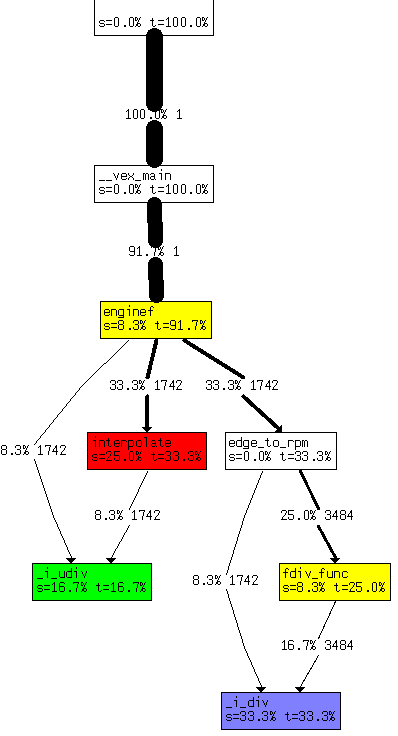
\includegraphics[width=\linewidth]{images/Engine-rgg.png}
    \subcaption{Engine: The call graph for the engine benchmark reveals that the benchmark performs a lot of divide operations (\_i\_div and \_i\_udiv). Figure made with gprof and rgg.}
    \label{fig:engine_call_graph}
\end{subfigure}%
\quad
\begin{subfigure}[b]{.495\textwidth}
  %\centering
      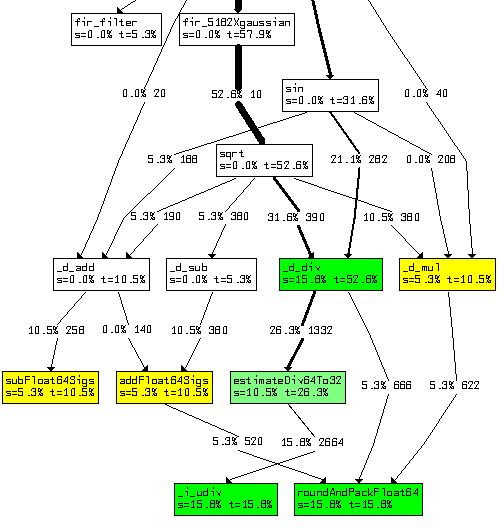
\includegraphics[width=\linewidth]{images/FIR-rgg3.png}
      \centering
    \subcaption{fir: The call graph for the fir benchmark reveals that the benchmark performs quite some divide operations (\_i\_udiv). Furthermore the add and subtraction operations, and the roundAndPackFloat are prominent.  Note that part of the graph is cut but that the nodes aren't relevant for show case of execution time as the relative execution time of those nodes (s) is zero. Figure made with gprof and rgg.}
    \label{fig:fir_call_graph}
\end{subfigure}
\end{figure}

\input{part2.tex}
\section{Configuration}
After a lot of experimentation the configuration file included with this report was created. In this section that configuration, the compiler flags and the process that led to the final result's will be discussed. Taking the amount of execution cycles shown in the ta.log file as the most important metric for performance (as advised), results in this section will often be compared to the original amount of execution cycles for the benchmarks (compiled with optimization level 3). These were 724703 and 509595 for engine and fir respectively.

\subsection{Clusters}
One of the first experiments was to see if there would be a significant difference between using the 1 cluster and 2 cluster example configurations. Confusingly, using an extra cluster seemed to barely have any effect on the performance of engine and even seemed to make fir slower. Taking a look at the assembly files for both revealed that fir barely used the second cluster. The inter cluster move operations may have been more taxing on the performance than the added benefit of using an extra cluster was making up for it. Unsurprisingly, significantly increasing the resources for both clusters did improve the performance. But still, while the performance increase for engine was pretty good (decreasing by as much as 60000 cycles of the original 725000 execution cycles), the performance of fir was barely impacted. A quick look in the fir.s assembly file confirmed that the second cluster was barely used. This is when it was decided that the processor was going to be designed using 1 cluster. The large amount of extra resources was not worth the increase in performance, considering that fir was barely affected. This also meant that \textbf{CopySrc} and \textbf{CopyDst} could be set to zero because no inter cluster communication was needed.

\subsection{Issue width, ALU, multiply}
Considering only one cluster was used, increasing the issue width was one of the first priorities so more instruction level parallelism could be achieved. Increasing the issue width to 8 and giving the processors more than enough resources in the ALU and multiply departments provided a significant improvement in performance for engine, and a slight improvement for fir. A look into the assembly files for both benchmarks did show that the bundles on average had become significantly bigger, but the full issue width was barely used making a smaller issue width of 4 also a sensible choice, slightly decreasing performance but saving a lot on resources.

Both programs seemed to not need a lot of multiplication so the amount of multiply syllables per cycle \textbf{Mpy} was set to 2. The amount of ALU syllables per cycle was kept high with \textbf{Alu} being set to 4 to allow the especially addition heavy engine (and somewhat less so fir) to keep it's execution cycles low.

\subsection{Memory and registers}
Considering that especially fir showed a lot of memory operations this is also an important part of the configuration file for performance. When the amount of connections to the data cache was put to 8 for both stores and loads up to 4 store and load syllables were showing up per bundle in the fir.s assembly file. Unfortunately this still accounted for only about 1000 execution cycles and engine didn't profit from it at all. Keeping that in mind it was decided to stick with \textbf{MemLoad} and \textbf{MemStore} both on 4 and the amount of allowed syllables per cycle (\textbf{Memory}) to 2.

A quick look at the assembly for both fir and engine showed that both (barely) didn't use r registers above 25 and b registers above 4. Therefore it was a quick decision to set \textbf{\$r} to 25 and \textbf{\$b} to 4.

\subsection{Compiler flags}
After editing the configuration file according as described above, the performance increase was not overwhelming. With engine at 652606 and fir at 506946 execution cycles it seemed that a better performance should still be possible. Therefore, a couple of compiler flags were used to increase performance. \textbf{-O4} was used in stead of optimization level 3 used in the lab manual but it didn't seem to have much effect. A very effective flag was \textbf{-fexpand-div}. \cref{ch:benchmarks} already showed that the function \_i\_div was used a lot in engine so using in-line assembly for these divisions was an obvious choice. Another very effective flag was \textbf{-autoinline}. Replacing function calls with the functions themselves it saved thousands of cycles for both engine and fir. Using the compiler flags brought the amount of execution cycles for engine down to 521269 and fir down to 472448.


\section{Environment}
\label{ch:environment}
The configuration for this processor is mainly for applications where power consumption is less important that raw performance.
Think bigger embedded systems (in vehicles for example) or desktops.
Especially fir which can be used for filtering applications.
When you need said function in a low power environment you will use a special function unit on the target device (DSP).
The functionality of engine would be use close to an actual engine, thus power is not a problem.
Most modern alternators deliver plenty of power to run even the biggest desktop size chips.
The trend in cars is towards more powerful hardware to enable all kinds of smart features.

The best performance was achieved using a single relatively big single cluster that is not terribly power efficient, but achieves high performance.
That especially in for example automotive can be crucial to bring latencies down and safety up.

\section{Conclusion}
A configuration for a processor was developed that not only significantly improves the performance of both benchmarks but also manages to stay relatively small. For engine the amount of execution cycles was brought down from 724703 to 521269 and fir from 509595 down to 472448. Improvements of respectively 29.7\% and 9.4\%. The improvement is significantly better for engine. Attempts at finding a configuration that had as shocking an improvement for fir as for engine were unsuccessful, though not for lack of trying. Of course, not every program leaves a lot of room for improvement. Some processes are inherently more sequential and therefore hard to improve by doing more work at the same time.

It should be noted that in the developing of this configuration a lot of priority was given to keeping the processor somewhat small and efficient. Possibly more so than was necessary for the environment laid out in \cref{ch:environment}. A slightly bigger performance improvement was still a possibility. Using an issue width of 8 with 6 ALU's and 4 multiply blocks yielded execution cycles of 517629 and 471082 for respectively engine and fir for example. Despite that, it was decided that the improvements weren't big enough to warrant an upgrade in size, cost and power consumption.


%\bibliographystyle{plain}
%\bibliography{references}
\end{document}
